\chapter{REASSEMBLE Case Study: Representation, Fusion, and Robustness}
On 4,530 completed robotic actions, the logistic stacker ranked failures better than the statistical sensor predictor (average precision 0.4473 versus 0.4294). Its advantage over equal averaging (0.4457) remained unresolved, and none of the original context-conditioned gates showed a consistent advantage. REASSEMBLE's paired video, machine signals and recorded outcomes made it possible to compare these methods on the same actions. Later experiments examined alternative representations and fusion rules on the same cohort.

The core experiment compared fusion models on a common prediction bank. The exploratory extensions and later visual studies used their own fitted models and assessed each change separately.\ev{Core study evidence}{\EvidenceRef{E044}{}}\ev{Visual fine-tuning experiments}{\EvidenceRef{E056}{}}

\begin{figure}[p]
\caption{Sampled Frames From a Completed REASSEMBLE Insertion}\label{fig:reassemble-example}
\centering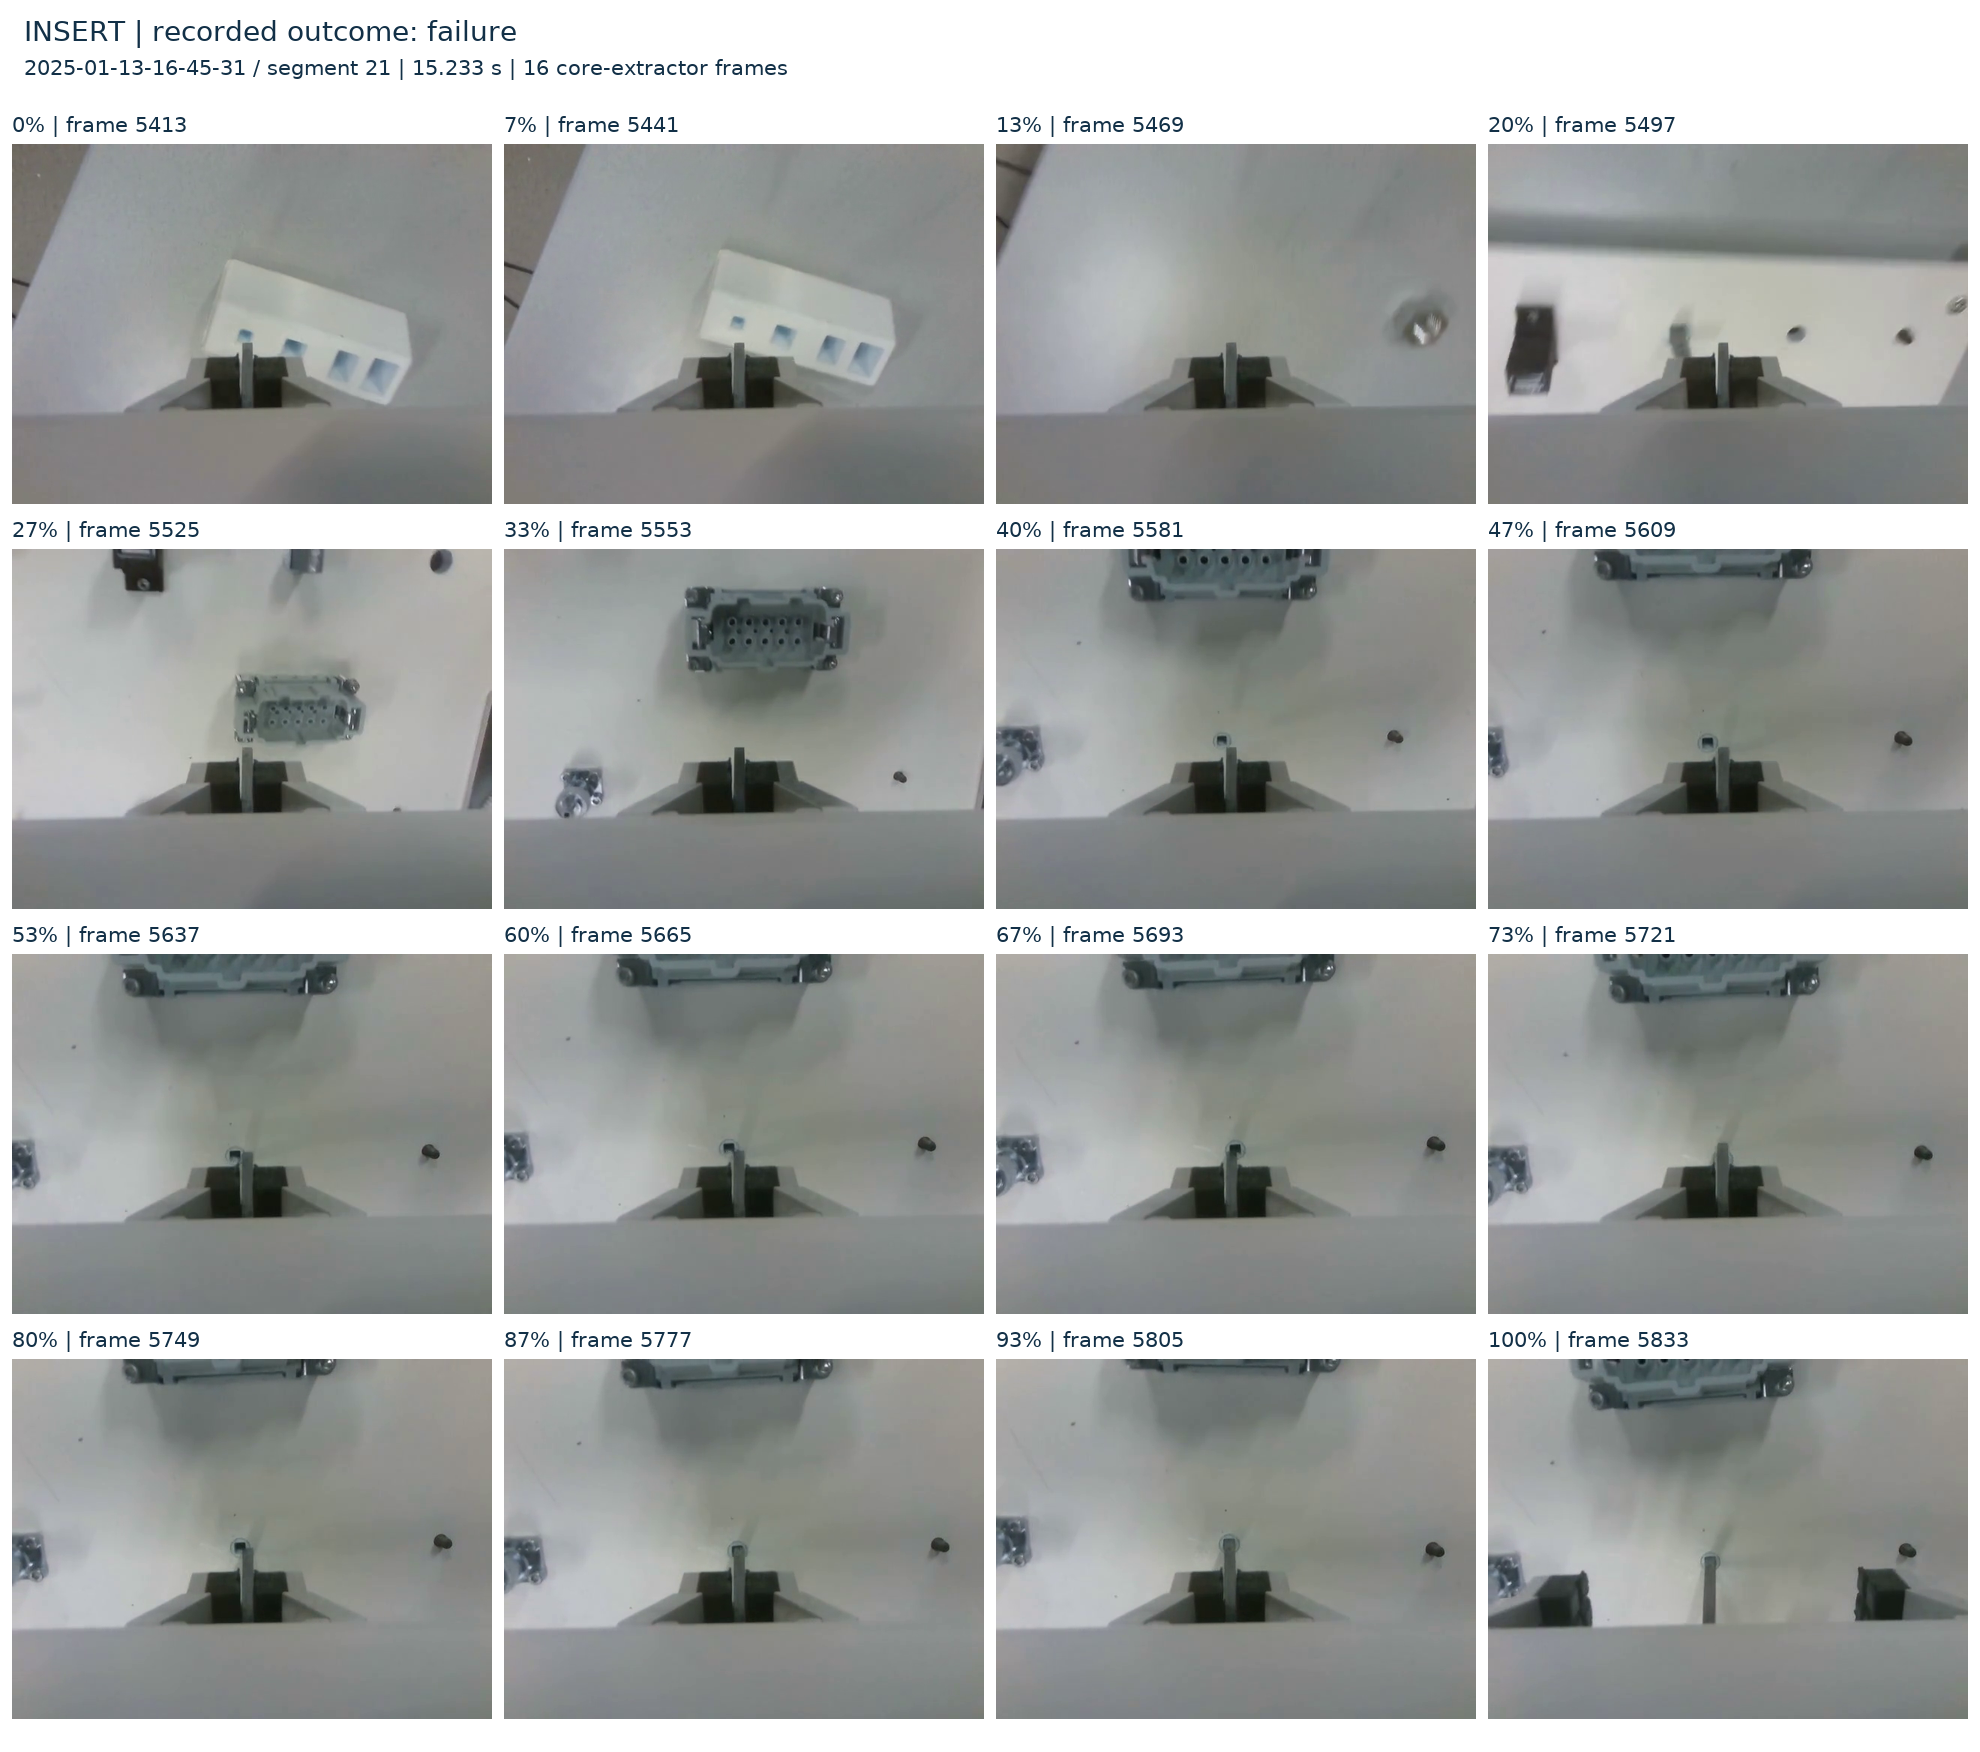
\includegraphics[width=\textwidth,height=.70\textheight,keepaspectratio]{figures/reassemble_example_frames.png}
\displaynote{The extractor selected 16 frames from recording 2025-01-13-16-45-31, segment 21 (15.233 s). The saved failure label accompanies this example. Frame selection illustrates temporal coverage. Source: Saved data-preparation example.}
\end{figure}
\ev{Illustrative frame source}{\EvidenceRef{E061}{}}
\section{Study Objectives and Research-Question Mapping}
SQ1 concerns implemented visual and temporal representations relative to engineered sensor statistics. SQ2 concerns early, late and adaptive fusion under shared recording groups. SQ3 distinguishes known missing modalities, synthetic degradation of a present modality and broader distribution shifts. SQ4 concerns the controls needed to interpret these comparisons: native labels, group separation, inner selection, calibration, paired uncertainty and computational budgets. The evaluation therefore includes simple reference predictors and a strong unimodal competitor before interpreting multimodal gains.

The task is retrospective classification of an already completed action. It is relevant to monitoring and automated inspection of industrial manipulation, but it is not a direct replication of rotating-machine damage diagnosis. The observation horizon includes the action's end. Consequently, a representation that exploits late frames can be useful here without demonstrating prediction before an unsuccessful event. The dataset paper supplies acquisition context; the retained manifests and implementation establish this thesis's specific population and task \parencite{Sliwowski2025REASSEMBLE}.\ev{Action targets and assessment cohort}{\EvidenceRef{E046}{}}

\section{Dataset Overview and Native Outcome Annotations}
The inventory contains 149 recordings; the retained common cohort contains 4,530 eligible actions from 148 recordings. A failure is one minus the native success indicator. There are 509 failures, giving positive-class prevalence 0.1124. Failure frequency differs substantially by action: pick has 98 failures in 1,190 actions; insert, 243 in 1,156; remove, 146 in 1,096; and place, 22 in 1,088. This makes action identity a substantive baseline. These filtered counts are distinct from the dataset paper's broader acquisition counts, because eligibility and task construction define the analysis population \citep{Sliwowski2025REASSEMBLE}.

The native outcome describes task success, not a spatial defect mask, severity score or verified physical root cause. One recording can contribute many actions, and actions from a recording share acquisition context. Counting 4,530 actions as independent experiments would overstate the amount of independent evidence. Recording identities are accordingly used for outer splitting and uncertainty resampling.\ev{Population and class counts}{\EvidenceRef{E046}{}}

\section{Dataset Challenges and Modality Availability}
The retained modalities are hand-camera images and machine-sensor measurements: three force channels, three torque channels, two gripper channels, seven joint-effort channels and seven joint-velocity channels. These twenty-two channels include operating state as well as direct interaction measurements. Complementarity is thus an empirical question, because both modalities may encode action identity or progress rather than independent evidence of failure.

Segment-offset and drift checks could not establish a common timing anchor for audio, so the predictive experiment excluded the audio branch. This is an alignment limitation, not a result showing that an audio model failed to learn. Similarly, seventeen object categories do not establish seventeen disjoint physical objects. The available relationship graph did not support a verified object-instance-disjoint test. The recording-disjoint split evaluates transfer between recordings. Generalization to unseen objects or sites and hardware-clock synchronization remain untested.\ev{Audio alignment and object-group feasibility}{\EvidenceRef{E044}{}}

\section{Preparation and Pre-Checks}
Preparation established a common cohort before comparing architecture outputs. Required information included native action boundaries and outcomes, valid camera correspondence, sufficient sensor coverage, and a recording-group identity. These checks support comparable inputs and prevent changing the evaluation population in response to a particular model's performance. They do not certify that every outcome label is unambiguous or that every sensor is physically calibrated.

Eligibility checks and representation choices are distinct: temporal pooling changes the view of an accepted action, whereas missing observations can affect eligibility or require a missingness policy.\ev{Preparation and common cohort}{\EvidenceRef{E046}{}}

\subsection{Cohort Construction and Exclusions}
The core analysis uses exactly 4,530 common eligible actions and retains one outcome per action. Inventory recordings and retained recordings are reported separately rather than treating the unused recording as evidence of unexplained model failure. Actions outside the four specified types or without usable required observations are outside this cohort. Exclusion manifests, rather than model-score thresholds, define eligibility.

Later studies sometimes assess only 753 of these actions. That population is the original outer-fold-zero assessment subset, containing 77 failures in 26 recordings; it is not a newly acquired independent holdout. Its prevalence, approximately 0.1023, differs from the complete cohort's prevalence. Because average precision depends on prevalence and population composition, a 753-action AP cannot be ranked directly beside a pooled 4,530-action AP as if only architecture had changed.\ev{Core cohort}{\EvidenceRef{E046}{}}\ev{Populations used in follow-up comparisons}{\EvidenceRef{E058}{}}

\subsection{Visual--Sensor Correspondence and Action Boundaries}
Sixteen distinct frames are selected deterministically at approximately uniform positions within each completed action. The selection uses the recorded action interval; it does not learn where failure begins. Sensor observations are associated with that same action and resampled to 512 normalized progress positions. These positions are not a 512-Hz sampling rate. Normalized progress enables fixed-shape fitting across different action durations while changing the temporal interpretation of features.

Checks establish manifest-level correspondence and acceptable available coverage. They do not prove sub-frame synchronization from a shared hardware clock. Boundary errors can affect both modalities jointly, and late visual information may reflect the already known outcome. The subsequent boundary review and temporal pooling experiment address parts of this problem, without converting the task into online warning.\ev{Input construction}{\EvidenceRef{E064}{}}\ev{Boundary-aware follow-up}{\EvidenceRef{E042}{}}

\subsection{Missing, Invalid, and Inconsistent Observations}
Sensor extraction requires at least 0.89 finite coverage per channel and avoids extrapolation and interpolation across long gaps. Accepted residual missing values are filled with training-partition means after channel standardization. Masks remain part of the input preparation, but the retained PatchTST configuration does not convert the observed mask into attention suppression. Passing a mask to an API and enforcing missing-token attention are therefore different claims.

Some proposed quality descriptors have limited information even on clean data. The gripper median-absolute-deviation outlier statistic is undefined for 1,562 rows and is imputed from training data; sixteen quality fields are constant. These details qualify the interpretation of a quality-aware gate: its input name alone does not establish that it receives a reliable independent quality estimate. Conversely, the deliberate complete-modality-loss experiments supply a known availability mask, which is stronger information than detecting an unnoticed hardware failure.\ev{Sensor preparation}{\EvidenceRef{E064}{}}\ev{Quality audit}{\EvidenceRef{E048}{}}

\subsection{Human Annotation Review and Its Limits}
One reviewer completed 64 selected clips. Of 59 determinate judgments, 57 agreed with the native outcome and two disagreed; five of 64 were indeterminate. Agreement among determinate cases is therefore 96.6\%, while agreement over all reviewed cases is 89.1\%. These denominators answer different questions. Sampling balanced action and label strata with recording spread rather than drawing an unstratified population sample, so neither proportion is an unbiased dataset-wide error estimate.

For action boundaries, sixty clips were acceptable, three questionable and one indeterminate; four possible presentation artifacts were also flagged. Overlapping flags identify ten unique clips requiring adjudication. A single reviewer completed the assessment. Inter-rater agreement and adjudicated outcomes are therefore unavailable. Labels, folds and model metrics consequently retain their original definitions; the review identifies specific uncertainties rather than supplying a replacement ground truth.\ev{Single-reviewer action and boundary judgments}{\EvidenceRef{E051}{}}

\subsection{Group Definitions and Split Checks}
Five outer folds hold out whole recordings, with four recording-disjoint inner folds for selection. Outer assessment populations contain 753, 964, 1,037, 906 and 870 actions; their failure counts are 77, 109, 125, 99 and 99, respectively. The corresponding recording counts are 26, 31, 32, 29 and 30. Summing the assessment rows recovers all 4,530 actions, 509 failures and 148 recordings exactly.

Within each outer training set, the visual and sensor branches supplied out-of-fold (OOF) predictions for training the logistic stacker. Each branch predicted an action using a fit that excluded its recording. During inner validation of the stacker, however, every split reused this bank. Some rows used to train the stacker could therefore come from branch fits that had seen recordings assigned to the stacker's inner validation split. This indirect dependency affects internal model and threshold assessment. It does not extend to the outer test: those recordings were excluded from branch fitting, calibration, stacker training and threshold selection. Fully independent inner validation would require rebuilding the branch prediction bank within every stacker-validation split, including repeated branch fits and calibration across all five outer folds. This additional nesting was beyond the training budget, so the outer scores evaluate the procedure that reused the outer-training bank.\ev{Dependencies in stacker validation}{\EvidenceRef{E004}{section 15.4}}

\section{Task Formulation, Model Inputs, and Shared Evaluation Protocol}
The positive class is failure. The principal ranking measure is average precision (AP), computed by the average-precision implementation rather than trapezoidal integration of a precision--recall curve. AUROC, balanced accuracy, macro-F1, failure recall and precision, Brier score and fifteen-bin equal-width expected calibration error (ECE) describe other aspects of performance. Precision--recall reporting is particularly important at the observed minority-class prevalence \parencite{Saito2015PrecisionRecall}.

Unless a later subsection states otherwise, reported core scores pool each action's outer-held-out probability across the five folds. Pooled AP is not the arithmetic mean of five fold AP values. Training-only selection and sigmoid logistic calibration use appropriate inner outputs. Hard-decision thresholds maximize inner balanced accuracy over 0.01--0.99, with ties resolved toward 0.5. Calibration and threshold selection are separate operations. Two thousand paired recording-cluster bootstrap resamples quantify uncertainty conditional on the retained fitted models; they do not refit the entire procedure or estimate all training-seed uncertainty. Nineteen structured label-shift permutations preserve recording/action structure under their conditional exchangeability assumption, giving a smallest plus-one probability of 0.05.\ev{Metrics and inference definitions}{\EvidenceRef{E046}{}}

\section{Experiment A: Unimodal Representations}
The unimodal study establishes a reference hierarchy before fusion. Class-prior, majority and action-type predictors reveal what can be achieved without detailed observations. Engineered sensor statistics are then compared with the frozen visual representation and a compact sensor Transformer. Identical retained action identifiers and recording groups prevent changes in population from masquerading as representation gains.\ev{Unimodal experiment}{\EvidenceRef{E046}{}}

\subsection{Objective and Comparison Rationale}
The unimodal comparison included simple predictors that can exploit process or sensor information beyond class prevalence. The action-type predictor controls for the large native failure-rate differences between pick, insert, remove and place. The sensor-statistics model controls for useful low-complexity descriptions of force, torque and motion. The two neural branches test different inductive biases within bounded budgets; they do not represent exhaustive optimization of all visual or time-series models.

Both neural branches improved AP over the action baseline. Their AUROC differences remained unresolved. A later test of incremental predictive value motivated the visual--sensor fusion comparison.\ev{Neural baselines and incremental fusion comparison}{\EvidenceRef{E047}{}}

\subsection{Visual Representation Configurations}
The core visual extractor loads the COCO-pretrained RT-DETR-R18vd checkpoint (\texttt{PekingU/rtdetr\_r18vd}) at the recorded revision. From the loaded detector instance, it selects \nolinkurl{wrapper.model.backbone.model}, the checkpoint's own ResNet18-vd CNN backbone, and freezes its parameters. The forward pass reads this backbone's feature maps and bypasses the hybrid Transformer encoder, detection decoder, and box heads \parencite{Zhao2024RTDETR}.

Frames are resized to $640\times640$ using bilinear interpolation, converted to RGB and divided by 255 without ImageNet mean/standard-deviation normalization. Spatial means from three scales concatenate to 896 features per frame; the sixteen frame descriptors are averaged. A frozen extractor feeds a $896\rightarrow128\rightarrow1$ ReLU/dropout head with 114,945 trainable parameters. Whole-action averaging discards temporal order. Weighted binary cross-entropy, AdamW with learning rate 0.001 and weight decay 0.001, batch size 128 and gradient clipping at one are used. Inner selection chooses five or ten epochs; outer budgets are 5, 5, 10, 10 and 5.\ev{Executed visual computation}{\EvidenceRef{E064}{}}\ev{Head and fitter}{\EvidenceRef{E065}{}}

\subsection{Statistical Sensor and PatchTST Configurations}
The statistical representation computes ten features per channel: mean, standard deviation, median, minimum, maximum, lower and upper quartiles, range, RMS and progress slope. Twenty-two channels therefore produce 220 features. A training-standardized, class-balanced L2 logistic model selects $C$ from 0.1, 1 and 10 by mean inner AP. A subsequent unweighted $C=1$ logistic sigmoid calibrates selected out-of-fold raw scores.

The neural branch is a scratch-trained Hugging Face PatchTST-style model with context $512\times22$, patch length 32, stride 16, hidden width 32, two layers, four heads and feed-forward width 64. Internal scaling is disabled; layer normalization and dropout 0.1 are used. Mean patch pooling and channel concatenation feed a 128-dimensional projection and binary head, giving 109,505 trainable parameters. The observed mask is passed but does not suppress attention in this configuration. Inner selection allows three or six epochs and chooses six in every outer fold. This is a compact adaptation of the patching idea, not a claim to reproduce all settings of the original PatchTST paper \parencite{Nie2023PatchTST}.\ev{Sensor classification architecture}{\EvidenceRef{E065}{}}

\subsection{Results and Computational Considerations}
Table~\ref{tab:reassemble-unimodal} reports pooled assessment scores. The majority predictor has AP equal to prevalence, while the action predictor improves ranking substantially. Sensor statistics are the strongest retained unimodal representation. Relative to statistics, PatchTST changes AP by $-0.1878$ with a paired 95\% interval $[-0.2314,-0.1407]$ and AUROC by $-0.0740$ $[-0.1004,-0.0469]$. Similar trainable head sizes therefore do not imply similar predictive utility.

\begin{table}[htbp]
\caption{Unimodal Predictions on REASSEMBLE}\label{tab:reassemble-unimodal}
\centering\small

\begin{tabular*}{\linewidth}{@{\extracolsep{\fill}}lrrrrr@{}}\toprule
Model & AP & AUROC & Recall & Brier & ECE\\\midrule
Majority & .1124 & .5000 & .0000 & .1124 & .1124\\
Action type & .1808 & .6851 & .7642 & .0951 & .0080\\
Sensor statistics & .4294 & .7793 & .6149 & .0804 & .0174\\
Frozen visual mean & .2307 & .6978 & .6621 & .0943 & .0070\\
Short-budget PatchTST & .2416 & .7054 & .5639 & .0937 & .0067\\\bottomrule
\end{tabular*}
\displaynote{Scores pool held-out predictions for 4,530 actions. Failure is the positive class.}
\end{table}

The AP intervals are $[.3801,.4828]$ for statistics, $[.1983,.2701]$ for vision and $[.2102,.2826]$ for PatchTST. The visual pipeline also includes video decoding and frozen CNN extraction, unlike fitting directly on compact statistics. In the retained warm-component benchmark, statistical sensors took 26.267 ms, vision 478.415 ms, F2 504.693 ms and F6 564.021 ms. These measurements used a T4, four CPU threads, three deterministic segments, sensor arrays in memory and cached compressed video; fusion times are sequential component sums. They establish a bounded practical cost difference rather than cold-start throughput or a real-time deployment guarantee. Counting only F2's three learned combination parameters would omit the branch heads and frozen visual backbone.\ev{Saved unimodal estimates}{\EvidenceRef{E046}{}}\ev{Bounded component timing}{\EvidenceRef{E043}{}}

\subsection{Interpretation and Implications for Fusion}
Visual AP exceeds the action reference by 0.0499 $[.0225,.0836]$, and PatchTST exceeds it by 0.0608 $[.0293,.0974]$. Their AUROC differences, 0.0127 $[-.0154,.0406]$ and 0.0203 $[-.0115,.0494]$, remain unresolved. These are metric-specific findings, not equivalence results. Lower neural AP than sensor statistics also does not exclude incremental information: useful errors can differ even when one standalone predictor is weaker.

The fusion experiment therefore uses the statistical sensor predictor as its reference. Each fitted fusion pipeline is compared with that predictor on the same held-out actions. The stacker also fits a new logistic map to the branch probabilities. The saved visual term's contribution to within-fold ordering is examined below. Attribution of the complete pooled gain remains limited by the absent matched sensor-only second-stage control. A separate follow-up tests how the training budget affects PatchTST performance.\ev{Paired unimodal and incremental fusion comparisons}{\EvidenceRef{E047}{}}

\section{Experiment B: Fusion Strategies}
Six fusion families share the cohort and recording structure: probability averaging, stacking, representation concatenation and three context-dependent gates. Their input spaces and calibration stages differ.\ev{Fusion experiment}{\EvidenceRef{E048}{}}

\subsection{Objective and Hypotheses}
The first hypothesis is that the combined visual--sensor pipeline improves held-out failure ranking relative to the retained sensor pipeline. The second is that action or quality context improves allocation between branches. These questions are distinct: a fixed map can use complementary predictions without an effective per-instance reliability estimate. The comparison changes both inputs and the fitted probability map. Within-fold ordering can nevertheless identify a visual contribution beyond a strictly increasing transformation of the sensor score. A matched sensor-only second-stage model, which was not completed, would strengthen attribution of the full pipeline contrast. Both sensor-only and simple static fusion references are therefore needed when interpreting adaptive models.

Clean gains do not establish corruption recognition; the subsequent experiment tests frozen clean-trained models directly.\ev{Fusion questions and controls}{\EvidenceRef{E048}{}}

\subsection{Compared Architectures and Exact Fusion Formulations}
F1 averages calibrated probabilities: $p=(p_v+p_s)/2$. F2 fits a fixed-$C=1$ L2 logistic stacker,
\begin{equation}p=\sigma(b+a_vp_v+a_sp_s).\end{equation}
It has three scalar parameters. Its signed coefficients are unconstrained and do not form convex reliability weights. F3 instead projects the 128-dimensional visual representation and 220 sensor statistics to separate 128-dimensional vectors, concatenates and layer-normalizes them, and uses a hidden layer of width 32 or 64. Candidate training budgets are ten or twenty epochs.

F4--F6 use a masked softmax gate and calibrated branch logits:
\begin{equation}w=\operatorname{softmax}(h(u)+\text{availability mask}),\qquad p=\sigma\!\left(\sum_m w_m\operatorname{logit}(p_m)\right).\end{equation}
F4 receives four action indicators and two availability indicators. F5 receives thirty-six quality descriptors and availability; F6 receives all forty-two inputs. Hidden widths are eight or sixteen. The gates have no final intercept correction or post-gate calibrator. Context or quality can encode process content as well as reliability; interpreting a learned weight as causal sensor trust is therefore unsupported.\ev{Exact implemented fusion links}{\EvidenceRef{E066}{}}

\subsection{Training, Calibration, and Evaluation}
Fusion uses branch prediction banks with recording-excluded row construction and held-out outer assessment recordings. The internal bank-reuse dependency described above remains part of its selection procedure. F2 stacks calibrated probabilities, whereas F4--F6 mix calibrated logits. F2 fixes $C=1$ and has no further calibration stage. F3 uses weighted binary cross-entropy and a sigmoid calibrator; the gates use unweighted binary cross-entropy, forty epochs, learning rate 0.003 and weight decay 0.001. These differences in link, objective and calibration opportunity are part of the recipes, rather than controls that isolate adaptation alone.

Gate results average probabilities from seeds 20260927--20260929. Averaging probabilities is not equivalent to inserting averaged weights into a sigmoid. The core threshold protocol and paired recording bootstrap remain in force. These controls improve comparability but do not equalize every architecture's effective capacity, objective or calibration opportunity.\ev{Fusion training and nested banks}{\EvidenceRef{E048}{}}

\subsection{Predictive Results and Uncertainty}
F2 has AP 0.4473 and AUROC 0.7950. The paired differences for F2 minus the statistical sensor predictor were 0.0179 $[.0086,.0283]$ in AP and 0.0156 $[.0060,.0255]$ in AUROC. The Brier score difference was $-0.0020$ (95\% CI $[-.0031,-.0009]$), indicating lower probability error for F2. The ECE difference $-0.0036$ $[-.0127,.0099]$ and recall difference $-0.0039$ $[-.0255,.0163]$ remain unresolved. The more precise AP contrast is $+0.017907$ $[.008603,.028284]$. Against probability averaging, F2's AP gain is only $+0.001556$ $[-.007607,.011165]$, which does not establish a discrimination advantage. Thus the retained evidence supports a modest combined-pipeline increment over sensors, with improved probability quality on some metrics, rather than a general superiority of learned stacking over simple averaging.

\begin{table}[htbp]
\caption{Fusion Results for the 4,530 Matched REASSEMBLE Actions}\label{tab:reassemble-fusion}
\centering\small

\begin{tabular}{lrrrrr}\hline
Model & AP & AUROC & Recall & Brier & ECE\\\hline
F1 probability mean & .4457 & .7951 & .6031 & .0834 & .0355\\
F2 probability stacker & .4473 & .7950 & .6110 & .0784 & .0138\\
F3 representation fusion & .4122 & .7856 & .6385 & .0827 & .0149\\
F4 action gate & .4437 & .7815 & .6031 & .0802 & .0128\\
F5 quality gate & .4445 & .7760 & .6012 & .0806 & .0126\\
F6 combined gate & .4414 & .7755 & .5717 & .0807 & .0124\\\hline
\end{tabular}
\end{table}

All three original gates have lower AUROC than F2, with intervals excluding zero for those differences. Their AP differences remain unresolved. The AP difference for F6 minus F2 was $-0.0059$ $[-.0248,.0137]$. The failure-recall difference for F6 minus F2 was $-0.0393$ (95\% CI $[-.0649,-.0122]$).\ev{Fusion results and paired contrasts}{\EvidenceRef{E048}{}}

\subsection{Modality Complementarity and Error Analysis}
At the frozen hard-decision thresholds, both unimodal branches are correct on 2,347 actions and both wrong on 529. Vision alone is correct on 486, while sensors alone are correct on 1,168. Among 509 failures, 240 are identified by both, 99 by neither, 97 by vision alone and 73 by sensors alone. Failures detected by vision alone occurred in 61 recordings.

An oracle that always selected a correct branch would identify 410 of 509 failures, approximately 0.8055 recall. That is an unavailable truth-dependent upper reference, not an achieved fusion result or a deployable gate. Complementarity provides potential information, while learning which branch to trust from available inputs remains a separate problem. These counts describe decisions at fixed thresholds. Paired AP comparisons assess the ranking of the same actions across thresholds.\ev{Error-overlap analysis}{\EvidenceRef{E047}{}}

\subsection{Interpretation and Comparison Limits}
Independent saved-prediction recomputation separates within-fold ordering from cross-fold score alignment. All five F2 sensor coefficients are positive. Omitting the visual term while retaining the jointly fitted parameters, $q_{s,k}=\sigma(b_k+\alpha_{s,k}p_s)$, therefore preserves sensor ordering within fold $k$. Its AP and AUROC match the sensor branch exactly within every fold. Restoring vision improves AUROC in all five folds and AP in four; the remaining AP difference is $-0.00469$. Thus, the visual term supplies beneficial observed ordering changes beyond a strictly increasing transformation of the same sensor probabilities, although its AP benefit is not uniform. Appendix~\ref{app:supplementary-results} gives the fold-level check.

Pooled AP is .42939 for sensors, .43092 for the reduced score and .44730 for complete F2. Different fold-specific maps can change pooled ordering while preserving every within-fold ranking. This omission is an arithmetic diagnostic, not a refitted sensor-only control or a missing-modality experiment. It does not uniquely allocate the pooled gain to vision, establish information conditional on all sensor features, or quantify causal modality importance. AP changes also do not measure calibration. The folds share training populations; historical recording-bootstrap intervals condition on fixed models and omit training and repeated selection uncertainty. These findings do not establish population-wide superiority or a resolved advantage over equal averaging.\ev{Independent saved-score verification}{\EvidenceRef{E113}{}}

Within the tested representations and budgets, neither intermediate fusion nor the original adaptive gates establishes an advantage over the successful static reference. This finding is architecture- and protocol-specific. The later anchored model changes the link and learns a different function class; its positive exploratory AP result is therefore compatible with the original gates' bounded negative evidence.\ev{Original REASSEMBLE fusion comparisons}{\EvidenceRef{E044}{}}

\section{Experiment C: Missing and Degraded Modalities}
The core robustness study froze the clean-trained statistical sensor and visual predictors (U1 and U2), equal averaging (F1), the stacker (F2), and the two gates using quality descriptors (F5 and F6). It perturbed one input at a time and also tested known loss of a full input stream.\ev{Core robustness study}{\EvidenceRef{E055}{}, \EvidenceRef{E049}{}}

\subsection{Robustness Questions and Tested Conditions}
The central question is whether a gate both changes allocation in the expected direction and limits predictive deterioration relative to F2. Absolute performance at high severity is also necessary: a weak clean model can show a small decline merely because little useful ranking remains to lose. An intact unimodal branch supplies a practical reference for whether fusion introduces avoidable damage.

Clean decision thresholds remain frozen during corruption. This matches a deployment in which the operator does not receive fault labels and recalibrate at every severity. Known availability masks in complete-dropout tests are an explicitly different information condition. The two sets of results measure responses to different information about the fault.\ev{Robustness contrasts and decision policy}{\EvidenceRef{E049}{}}

\subsection{Corruption Operators and Severity Definitions}
Visual operators include pixel Gaussian noise with standard deviations 0.02, 0.05 and 0.10 on the normalized scale, Gaussian blur at severities one, two and four, and removal of two, five or eight of sixteen selected frames. Sensor operators include Gaussian noise scaled by 0.1, 0.5 or 1.0 training-channel standard deviations; removal of two, seven or eleven channels; missing temporal blocks covering 10\%, 30\% or 50\% of the sequence; and six force/torque channels stuck at training medians.

Sensor statistics and quality descriptors are recomputed from the altered input, rather than retaining clean summaries beside corrupted signals. The core uses its fixed operator realization protocol. A later augmentation study averages across five stochastic test realizations. Its Gaussian-noise estimates therefore refer to a different evaluation protocol. None of these operators is direct evidence of cross-machine shift, clock drift or physical sensor recalibration.\ev{Operator implementation and severities}{\EvidenceRef{E049}{}}

\subsection{Missingness Policies and Dropout Experiments}
In the original complete-dropout test, the four evaluated fusion models used the statistical sensor probability and threshold when vision was absent. When sensors were absent, they used the visual predictor and its threshold. The evaluator received the identity of the missing stream. The core gate rejects a sample with both streams absent. The robustness report contains no empirical result for that condition. A later quality-interaction pilot marked such predictions unavailable.

A separate F6 training experiment samples visual-only dropout with probability 0.15, sensor-only dropout with probability 0.15 and both-present inputs with probability 0.70. Both-absent inputs are never sampled. Because a one-available-modality softmax has weight exactly one and the branches are fixed, its missing-case output is structurally fixed and supplies no useful gradient for improving the fallback prediction. Dropout training cannot make that output better under this architecture. Its clean AP is 0.4377, changing ordinary F6 by $-0.0037$ $[-.0085,.0003]$.\ev{Explicit fallback and dropout}{\EvidenceRef{E045}{}}

\subsection{Predictive Performance and Calibration Under Degradation}
Under strongest pixel Gaussian noise, F2 retains AP 0.3963, while F5 and F6 fall to 0.1288 and 0.1275. The intact sensor baseline remains at AP 0.4294. F2's Brier score nevertheless rises to 0.2968 and ECE to 0.4368, compared with clean sensor values 0.0804 and 0.0174. Ranking retention therefore conceals severe probability failure.

Under sensor Gaussian noise at one training standard deviation, F2 AP is 0.2222 and F5/F6 are 0.1753/0.1788, below intact vision at 0.2307. F2's Brier/ECE rise to 0.4798/0.5251. Strong blur gives F2/F5/F6 AP 0.4099/0.4061/0.4179, without a resolved general gate advantage. These conditions demonstrate that combining an intact and corrupted modality can underperform the intact branch. Detection of corruption and calibrated uncertainty remain unresolved rather than being supplied automatically by a fusion layer.\ev{Core high-severity metrics}{\EvidenceRef{E049}{}}

\subsection{Gate Behaviour and Fallback Behaviour}
No tested original gate/family combination establishes both an appropriate allocation response and a smaller decline under the study's criteria; no supported absolute high-severity AP superiority follows. A gate weight can change with a quality input without changing in a beneficial way. Conversely, a smaller performance decline from a weaker clean starting point is insufficient to establish improved reliability.

Exact missing-modality equality follows programmed fallback. It demonstrates consistent handling of known absence, while corruption recognition and useful recovery remain separate capabilities. This is narrower than training an encoder or student to retain performance after input loss, as in transferable missing-modality methods \citep{P005,P007,P016}.\ev{Gate allocation and fallback audit}{\EvidenceRef{E049}{}}

\subsection{Interpretation and Untested Conditions}
The core evidence rejects a broad claim of reliable adaptation for the tested gates. The AP, calibration and intact-branch comparisons capture different consequences of corruption. Robustness to known complete absence is largely architectural here; robustness to unnoticed corruption is empirically weak.

Natural missingness mechanisms, simultaneous partial failures, asynchronous clocks, new machines, new operating sites and prospective early warning were not established. The later augmentation study changes training exposure and tests several held-out operator families, but the same recording population and already observed core faults limit claims of independent discovery. An untested condition remains open rather than receiving a favorable interpretation from the model's name.\ev{Tested missingness and corruption conditions}{\EvidenceRef{E044}{}}

\section{Follow-up Investigations}
Three exploratory comparisons on the same cohort yielded higher average precision under their respective protocols. Last-quarter visual pooling with static stacking reached 0.4934, anchored adaptation reached 0.4683, and combining long-budget PatchTST with sensor statistics reached 0.4403. Each had its own control. The temporal-pooling study was completed separately from an earlier visual experiment that stopped after partial execution. Other follow-ups examined matched corruption exposure and visual tuning.\ev{REASSEMBLE follow-up experiments}{\EvidenceRef{E040}{}}

\subsection{Longer Sensor Training and Alternative Sensor Representations}
The longer-budget experiment retains the PatchTST inputs and architecture, permits up to one hundred epochs, and uses minimum ten epochs with patience twelve. No long-budget inner fit reaches the cap; outer budgets use rounded median inner best epochs. Against a matched short-budget control, AP rises from 0.2557 to 0.2853, a difference of 0.0297 $[.0122,.0451]$. The original short-budget experiment yielded 0.2416 AP under its own protocol.

Long training remains below statistics: AP difference $-0.1441$ $[-.1861,-.1009]$. A fixed-$C=1$ stacker combining long PatchTST and statistics reaches AP 0.4403, improving statistics by 0.0110 $[.0054,.0181]$. This combines two representations of the same sensor modality. It qualifies the original budget-dependent neural result while preserving the strong engineered baseline.\ev{Matched sensor-budget experiment}{\EvidenceRef{E040}{}}

\subsection{Alternative Visual Pooling}
The boundary-aware experiment exactly reproduces the original whole-segment mean before changing pooling. AP is 0.2556 for two halves, 0.3080 for thirds, 0.3191 for the last quarter, 0.2922 for early-plus-late and 0.2250 for an ordered GRU. The original mean is 0.2307. Last-quarter minus mean AP is 0.0885 $[.0424,.1293]$; the protocol's simultaneous lower bound across five AP contrasts remains positive at 0.0301.

This supports selected temporal aggregation changes, not a general recurrent-model advantage or an isolated causal effect of temporal order. The GRU changes capacity and inductive bias, while bin concatenation changes classifier inputs. The selected last-quarter rule exploits complete-action information. Its separate F2 follow-up reaches AP 0.4934, with the more precise value 0.493437 versus original F2 0.447299: difference $+0.0461$ $[.0260,.0632]$, and AUROC difference $+0.0403$ $[.0291,.0522]$. This is a meaningful exploratory same-cohort result after representation selection, not independent confirmation or warning before the outcome. It was not combined with the anchored adaptive gate or the same-sensor hybrid.\ev{Visual pooling definitions and paired comparisons}{\EvidenceRef{E042}{}}

\subsection{Spatial-Encoder and Backbone Comparisons}
A separate five-fold comparison tests CNN-only against CNN plus the spatial hybrid encoder, with the same sixteen frames, 4,530 actions, frozen extraction and five-epoch heads. It uses its own fitting and calibration subsets. CNN-only visual AP is 0.221644 and F2 AP 0.440764; hybrid-encoder visual AP is 0.171915 and F2 AP 0.424979, with shared sensor AP 0.420926. The hybrid-minus-CNN F2 difference is $-0.015785$ $[-0.024804,-0.005800]$. Executing more of the detector therefore worsens this particular comparison, rather than automatically improving representation quality.\ev{Matched spatial-component results}{\EvidenceRef{E039}{}}

The descriptors also differ in width: CNN multiscale pooling yields 896 features and the spatial hybrid-encoder path 768. Head size, active components and compute change with that representation. The result cannot isolate an attention effect, and the attention is spatial rather than across video time. Neither path executes the object-detection decoder. CNN-only extraction, spatial-encoder extraction, final-stage tuning and complete detector training remain distinct interventions.\ev{Architectures in the spatial-component comparison}{\EvidenceRef{E057}{}}

\subsection{Frozen Versus Fine-Tuned Visual Representations}
A matched two-epoch diagnostic uses thirty-two frames for both frozen and final-stage-tuned arms across the full 4,530-action cohort. It covers two seeds, with seventy-five newly executed and twenty-five reused fits. Epoch matching does not imply compute matching. Its fixed sensor recipe has pooled AP 0.4208, distinct from the core selected-$C$ baseline's 0.4294.

For seed 42, visual AP changes from 0.2227 to 0.2306, but the difference 0.0079 has interval $[-.0173,.0332]$; F2 changes from 0.4394 to 0.4386. For seed 20261023, visual AP changes from 0.2168 to 0.2005, and F2 from 0.4352 to 0.4324. The corresponding paired intervals include zero. These results do not identify a unique cause for the absence of a fusion gain, such as calibration or out-of-fold mismatch; two seeds also do not fully characterize seed variability.\ev{Matched two-epoch diagnosis}{\EvidenceRef{E062}{}}

The later twenty-epoch visual cap completes twenty inner and five outer fits for seed 42. Pooled visual AP is 0.3121, while mean fold AP is 0.3086. The additional fifty fits for two more seeds are deferred; their absence is not a failure of the twenty-five completed fits. Twenty-epoch F2 was not executed because its controller expected the larger bank. A current checkpoint validator's twenty-five-source-epoch requirement conflicts with the twenty-epoch donor; that is an eligibility/configuration conflict, not evidence of failed training.\ev{Completed twenty-epoch fits}{\EvidenceRef{E059}{}}

The hundred-epoch pilot restarts both arms from pretrained weights with fresh heads, rather than continuing the twenty-epoch run. Both arms execute one hundred epochs and select epochs fourteen (frozen) and forty-seven (full). On the same 753-action assessment subset, visual AP is 0.1938/0.2126 and F2 AP 0.3350/0.3491. Full-minus-frozen F2 AP is 0.0141 $[-.0008,.0291]$, leaving the difference unresolved. Restricted historical F2 is 0.3672 on these same rows; its full-cohort AP is not the relevant comparator.\ev{Matched pilot assessment cohorts}{\EvidenceRef{E058}{}}

\subsection{Adaptive-Fusion Extensions and Matched Controls}
Anchored adaptation preserves the successful F2 link and learns bounded adjustments:
\begin{equation}p=\sigma\!\left(b+\sum_m a_m[1+\tanh(h_m(u))]p_m\right).\end{equation}
The adaptive network is $42\rightarrow16\rightarrow2$ with zero final-layer initialization; a two-parameter constant adjustment is a matched control. AP reaches 0.4683, improving the matched anchor by 0.0210 $[.0015,.0419]$ and the constant adjustment by 0.0226 $[.0036,.0432]$. AUROC gains remain unresolved; recall falls and ECE rises relative to the anchor. Threshold differences also prevent treating its hard decisions as identical to historical F2. This is evidence for a particular exploratory function class, not retrospective success of F6.

Matched augmentation uses 50\% clean, 25\% pixel-noise and 25\% sensor-noise training views, recomputing quality without a supplied fault identity. The principal adaptive-minus-static contrast over six seen-family conditions is AP $+0.0097$ $[-.0034,.0228]$, unresolved. Strong blur gives adaptive AP 0.3968 versus static 0.4256; eleven dropped channels give 0.2128 versus 0.2924. Sensor Gaussian noise at one training standard deviation favors augmented adaptation, 0.2081 versus augmented static 0.1749, but clean-trained F2 is 0.2246 under this later realization protocol. These selective wins do not establish general robustness, and none of the clean noninferiority claims passes the specified 0.01 margin.\ev{Anchored and augmented controls}{\EvidenceRef{E040}{}}

A later observable-quality pilot uses the selected frozen16 recipe on 753 actions, with 77 failures in 26 recordings. Its historical static clean AP is 0.307929; the changed branch, training and calibration recipe distinguishes this value from the restricted original F2 and the hundred-epoch screen. It matches augmentation exposure across three heads: static A, additive-quality B and probability--quality interaction C. All use 3,777 OOF parent actions and 11,331 augmented rows, weighted 0.50 clean, 0.25 visual fault and 0.25 sensor fault per parent. Eight quality proxies enter the relevant models; A, B and C have 3, 11 and 27 parameters. C has unrestricted interaction and direct quality coefficients, rather than convex reliability weights.

The primary mean AP across declared Gaussian conditions is 0.253996 for A, 0.237360 for B and 0.257009 for C; clean AP is 0.307397, 0.292965 and 0.312168. C minus A is $+0.003012$ $[-0.026711,+0.032165]$ for the primary mean and $+0.004771$ $[-0.034258,+0.044544]$ clean. Neither robustness superiority nor clean preservation at the pilot's zero-loss margin is established. B minus A deteriorates by $-0.016636$ $[-0.030676,-0.002429]$ in a secondary contrast on the primary metric. The primary average covers repeats, severities and two Gaussian families; it is not AP computed after pooling repeated versions as independent subjects. Complete absence routes all heads identically to the survivor, while both absent yields unavailable predictions. Quality can encode action content as well as error risk, and the different capacities plus absent quality-only/content-matched controls leave the reliability mechanism unresolved.\ev{Augmentation-matched quality-interaction results}{\EvidenceRef{E038}{}}

\subsection{Resource-Constrained Screens and Their Interpretation}
The hundred-epoch pilot uses mutually disjoint roles: 1,752 training, 419 validation, 686 calibration, 920 inner-bank and 753 assessment actions, summing to the common 4,530 population. Their recording counts are 60, 15, 19, 28 and 26. Saved prediction action identifiers take precedence over a stale metadata field listing inner-bank recordings as assessment recordings. This correction changes interpretation of provenance, not the saved scores.

The full hundred-epoch arm records about 23.96 training hours and 25.82 active process hours. The twenty-epoch cap records about 126.23 training hours across twenty-five fits; 137.47 hours includes validation/inference. Different accounting units and populations prevent treating these totals as intrinsic model costs. Removed derived caches also make a cold reproduction differ from historical cached timing. The completed subset screen supplies a bounded paired comparison, while five-fold or multi-seed performance requires the corresponding predictions.\ev{Measured training and process times}{\EvidenceRef{E060}{}}\ev{Sample allocation by fitting role}{\EvidenceRef{E058}{}}

\section{Study Synthesis and Remaining Questions}
The follow-ups distinguish representation suitability, complementary information and fusion effectiveness. Longer PatchTST training improves AP by .0297 (95\% recording-bootstrap CI [.0122, .0451]) but remains .1441 below statistics. Insufficient training therefore contributes to the initial gap without fully explaining it under this recipe. Yet their same-sensor combination improves on statistics by .0110 [.0054, .0181]. A weaker standalone representation can retain useful complementary predictions; this is not fusion of two sensing modalities.

Last-quarter visual pooling raises AP by .0885 [.0424, .1293] with the same fitted head size as whole-action pooling. Additional head parameters cannot explain that contrast. Concentrated outcome cues or reduced dilution are plausible explanations, but neither was isolated, and the observation still extends to completion. The selected pooling variant also improves its separate F2 comparison by .0461 [.0260, .0632]. The spatial-encoder and matched adaptation studies show that additional processing or updated weights need not improve the downstream combination; inconclusive adaptation intervals do not establish equivalence.

Core F2 includes verified within-fold visual ordering gains, while its advantage over averaging remains unresolved. Anchored adjustment improves clean AP over its anchor and a constant-adjustment control, but lower recall and higher calibration error qualify the gain. Matched corruption exposure leaves the principal adaptive robustness effects unresolved. Changing coefficients therefore does not establish recognition of unreliable inputs. Known absence is separate: the common routing rule fixes the surviving prediction.

These interventions were assessed separately on an already examined population. No run combines boundary pooling, the same-sensor hybrid and anchored adaptation. Their strongest individual results do not define an evaluated final architecture. New recordings, natural faults, earlier prediction horizons and uncertainty beyond the fixed fits remain open.\ev{Controlled follow-ups and uncertainty}{\EvidenceRef{E040}{}, \EvidenceRef{E042}{}, \EvidenceRef{E062}{}, \EvidenceRef{E113}{}}
